%Poster template for use by PCFC / HGD / SWL, etc. (Prof. K. Alexander Heufer)
%Developed by Mark E. Fuller from examples and miscellany produced at RWTH Aachen
%(probably mostly from the work of Philippe Dreuw and Thomas Deselaers)
%This template copyright Mark E. Fuller, 2021 (mark.e.fuller@gmx.de)

\documentclass[final,hyperref={pdfpagelabels=false}]{beamer}
\usepackage{grffile}
\mode<presentation>{\usetheme{PCFCposter}}
%\usepackage[ngerman]{babel}        % Deutsch, neue Rechtschreibung
\usepackage[english]{babel}       % English  
\usepackage{csquotes}
\usepackage[utf8]{inputenc}
\usepackage{amsmath,amsthm, amssymb, latexsym}
\boldmath
\usepackage[orientation=portrait,size=a0,scale=1.4,debug]{beamerposter}

\usepackage{array,booktabs,tabularx}
\newcolumntype{Z}{>{\centering\arraybackslash}X} % centered tabularx columns
\newcommand{\pphantom}{\textcolor{white}} % phantom introduces a vertical space in p formatted table columns??!!

\listfiles
\usepackage{graphicx}
\usepackage{multicol}
\usepackage[version=3]{mhchem} % Formula subscripts using \ce{}
\newcommand{\nox}{NO$_x$} % our abbreviation
\usepackage{subfigure}

\usepackage[
backend=biber,
doi=true,
sorting=none,
sortcites=true,
maxbibnames=3,
minbibnames=1,
maxcitenames=2,
mincitenames=1,
citestyle=numeric-comp,
giveninits=true,
isbn=false,
date=year
]{biblatex}
\addbibresource{../sample.bib}

%%%%%%%%%%%%%%%%%%%%%%%%%%%%%%%%%%%%%%%%%%%%%%%%%%%%%%%%%%%%%%%%%%%%%%%
%                              @article
%%%%%%%%%%%%%%%%%%%%%%%%%%%%%%%%%%%%%%%%%%%%%%%%%%%%%%%%%%%%%%%%%%%%%%%
\DeclareBibliographyDriver{article}{%
	\usebibmacro{bibindex}%
	\usebibmacro{begentry}%
	\usebibmacro{author/translator+others}%
	\newunit\newblock%
	\setunit*{\addspace}%
	\usebibmacro{doi+eprint+url}%
	\usebibmacro{finentry}
}

% Make sure that URL is not printed if DOI is available
\renewbibmacro*{doi+eprint+url}{%
	\iftoggle{bbx:doi}
	{\iffieldundef{url}{\printfield{doi}}{\iffieldundef{doi}{}{\printfield{doi}}}}
	{}%
	\newunit\newblock
	\iftoggle{bbx:eprint}
	{\usebibmacro{eprint}}
	{}%
	\newunit\newblock
	\iftoggle{bbx:url}
	{\iffieldundef{doi}{\usebibmacro{url+urldate}}{}}
	{}
}

% New macro for @software to print both URL and DOI
\newbibmacro*{doi+url+software}{%
	\iftoggle{bbx:doi}
	{\printfield{doi}}{}%
	\newunit\newblock
	\iftoggle{bbx:url}
	{\usebibmacro{url+urldate}}{}%
}

%%%%%%%%%%%%%%%%%%%%%%%%%%%%%%%%%%%%%%%%%%%%%%%%%%%%%%%%%%%%%%%%%%%%%%%%%%%%%%%%%%%%%%
 
\title{\huge Reaction Class-Based {CHON} Combustion Mechanism Development}
\author{\LARGE Mark E. Fuller$^1$, K. Alexander Heufer$^1$}
\date{}
\institute{\Large $^1$Physico-Chemical Fundamentals of Combustion\\RWTH Aachen University}

%%%%%%%%%%%%%%%%%%%%%%%%%%%%%%%%%%%%%%%%%%%%%%%%%%%%%%%%%%%%%%%%%%%%%%%%
\begin{document}
\begin{frame} %whole poster is one frame

	\begin{columns}[T] %top-align
	\begin{column}{.48\textwidth}
		\begin{beamercolorbox}[center,wd=\textwidth]{postercolumn}
			\begin{block}{\LARGE Introduction}
				\begin{itemize}
					\item Interactions of \nox\ (\ce{NO} and \ce{NO2}) with the combustion
process are increasingly relevant in engines with exhaust gas
recirculation (EGR) and/or alkyl nitrate cetane enhancers
					\item Low-temperature combustion reactions with nitrogen are not
well-studied and may have significant effects
					\item Sustainable fuels, produced from bio-based carbon
feedstocks, \ce{CO2} , and renewable electricity, contain additional
functional groups whose reactions with \nox\ are not well-characterized
				\end{itemize}
			\end{block}
		\end{beamercolorbox}
	\end{column}
	% end left column
	% ---------------------------------------------------------%
	% start right column
	\begin{column}{.48\textwidth}
		\begin{beamercolorbox}[center,wd=\textwidth]{postercolumn}
			\begin{block}{\LARGE Model Development}
				\begin{itemize}
					\item Pentane isomer mechanism (\ce{CHO}) of Bugler {\it et al.} utilized as \ce{C0}-\ce{C5} base mechanism
					\item A sample citation\cite{Fuller.2014}
				\end{itemize}	
			\end{block}
		\end{beamercolorbox}
	\end{column}
\end{columns}

%fullwidth block
\begin{columns}
	\begin{column}{.98\textwidth}
		\begin{beamercolorbox}[center,wd=\textwidth]{postercolumn}
			\begin{block}{\LARGE Modeling results}
				\begin{multicols}{2}
					\begin{figure}
						\centering
						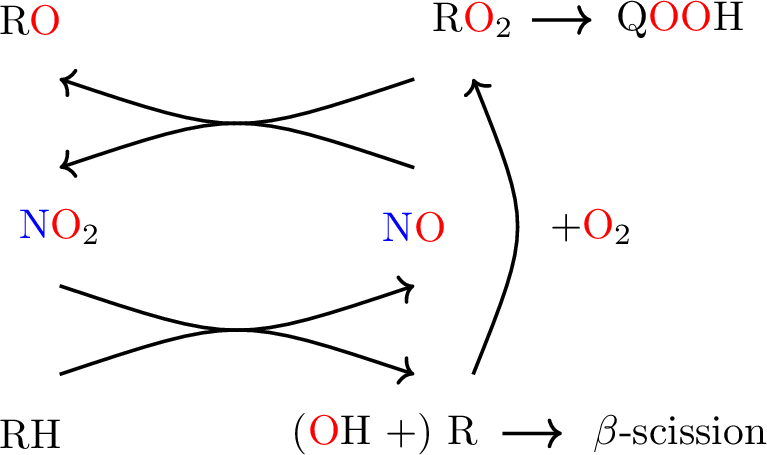
\includegraphics[width=0.8\linewidth]{../figures/NOx_cycle.png}
					\end{figure}
					\centering
					WOW!
					\columnbreak
					\begin{figure}
						\centering
						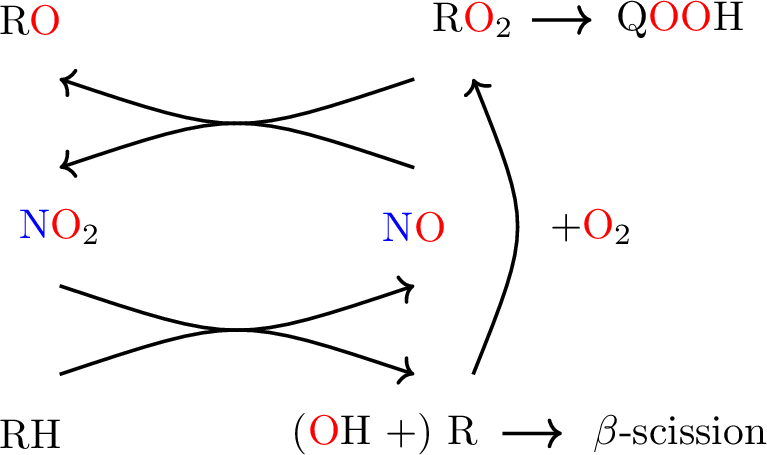
\includegraphics[width=0.8\linewidth]{../figures/NOx_cycle.png}
						\caption{Check this shit out!}
					\end{figure}
				\end{multicols}
			\end{block}
			%\vfill
		\end{beamercolorbox}
	
		\begin{beamercolorbox}[center,wd=\textwidth]{postercolumn}
		\begin{block}{\LARGE Rapid Compression Machine (RCM)}
			\begin{multicols}{3}
				\begin{figure}
					\centering
					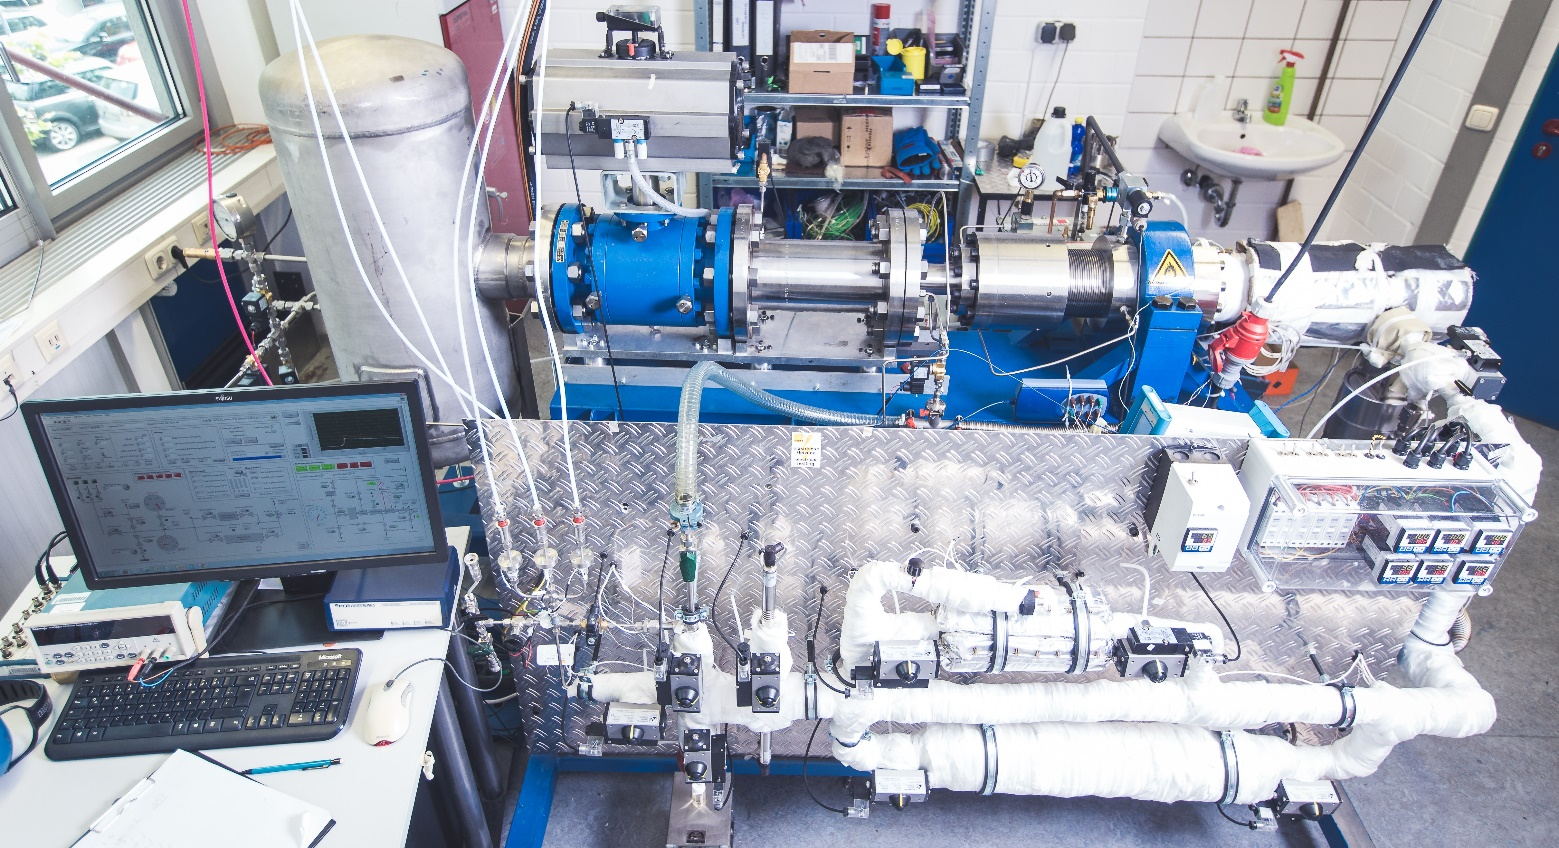
\includegraphics[width=0.96\linewidth]{../figures/PCFC_RCM.jpg}
					\caption{PCFC RCM Facility}
				\end{figure}
				\columnbreak
				\begin{figure}
					\centering
					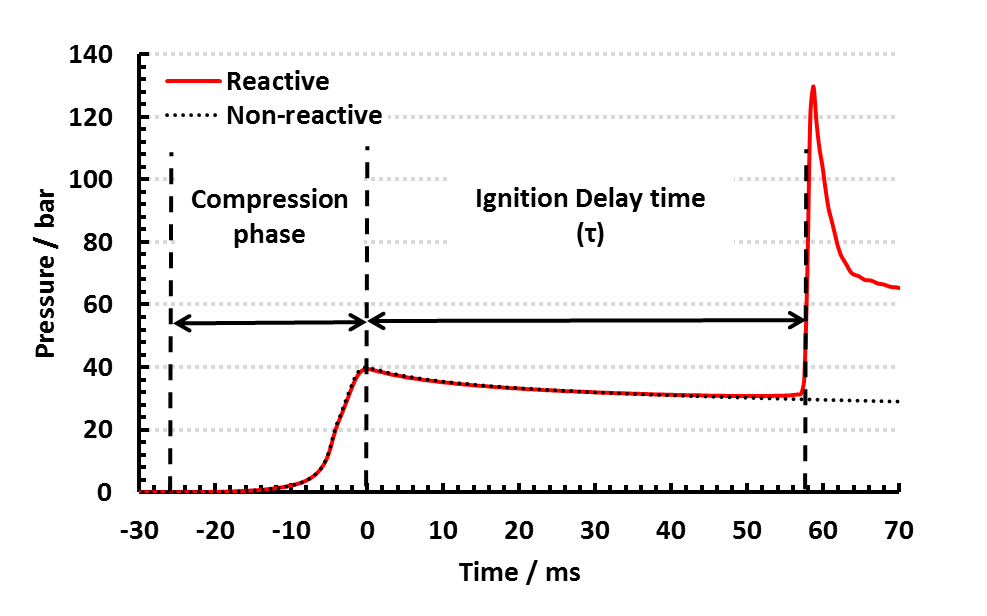
\includegraphics[width=0.96\linewidth]{../figures/RCM_typical.png}
					\caption{Characteristic RCM ignition experiments}
				\end{figure}
				\columnbreak
				\null \vfill
				\begin{itemize}
					\item Ignition delay time (IDT) measurements 2 to 200 ms
					\item Variable compression ratio 9 - 32
					\item End-of-compression pressure up to 100 bar, peak 1000 bar allowed
				\end{itemize}
				\vfill \null
			\end{multicols}
		\end{block}	
	\end{beamercolorbox}

	\end{column}
\end{columns}

%back to left /right columns
\begin{columns}[T] %top-align
	\begin{column}{.48\textwidth}
		\begin{beamercolorbox}[center,wd=\textwidth]{postercolumn}
			\begin{block}{\LARGE Work-in-progress}
				{\it Ab initio} calculations	
			\end{block}
		\end{beamercolorbox}
	\end{column}
	% end left column
	% ---------------------------------------------------------%
	% start right column
	\begin{column}{.48\textwidth}
		\begin{beamercolorbox}[center,wd=\textwidth]{postercolumn}
			\begin{block}{\LARGE REFERENCES}
				\printbibliography	
			\end{block}
		\end{beamercolorbox}
	\end{column}
\end{columns}
\vskip2ex



\end{frame}
\end{document}


%%%%%%%%%%%%%%%%%%%%%%%%%%%%%%%%%%%%%%%%%%%%%%%%%%%%%%%%%%%%%%%%%%%%%%%%